\documentclass{standalone}
\usepackage{tikz}
\usetikzlibrary{patterns, positioning}
\usetikzlibrary{shapes.misc}
\usepackage[outline]{contour}
\contourlength{1.5pt} 


\begin{document}
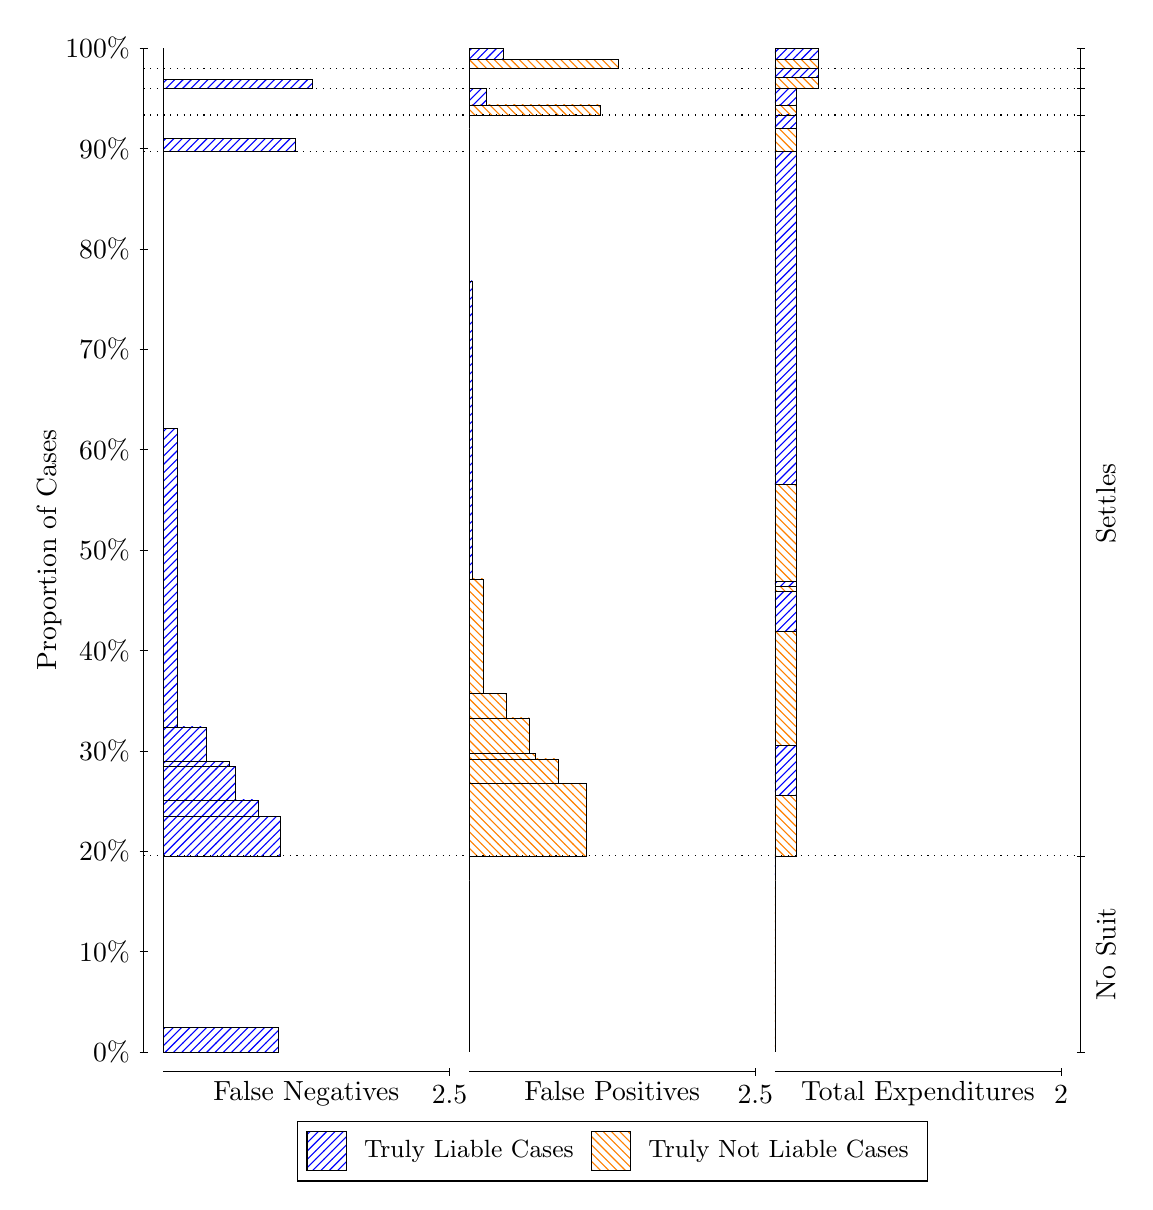
\begin{tikzpicture}
\draw[black, very thin] (1.5,1.75) -- (1.5,14.5);
\node[rotate=90, text=black, anchor=center] at (0.3, 8.125) {Proportion of Cases};
\draw[black, very thin] (1.45,1.75) -- (1.55,1.75);
\node[text=black, anchor=east] at (1.45, 1.75) {0\%};
\draw[black, very thin] (1.45,3.025) -- (1.55,3.025);
\node[text=black, anchor=east] at (1.45, 3.025) {10\%};
\draw[black, very thin] (1.45,4.3) -- (1.55,4.3);
\node[text=black, anchor=east] at (1.45, 4.3) {20\%};
\draw[black, very thin] (1.45,5.575) -- (1.55,5.575);
\node[text=black, anchor=east] at (1.45, 5.575) {30\%};
\draw[black, very thin] (1.45,6.85) -- (1.55,6.85);
\node[text=black, anchor=east] at (1.45, 6.85) {40\%};
\draw[black, very thin] (1.45,8.125) -- (1.55,8.125);
\node[text=black, anchor=east] at (1.45, 8.125) {50\%};
\draw[black, very thin] (1.45,9.4) -- (1.55,9.4);
\node[text=black, anchor=east] at (1.45, 9.4) {60\%};
\draw[black, very thin] (1.45,10.675) -- (1.55,10.675);
\node[text=black, anchor=east] at (1.45, 10.675) {70\%};
\draw[black, very thin] (1.45,11.95) -- (1.55,11.95);
\node[text=black, anchor=east] at (1.45, 11.95) {80\%};
\draw[black, very thin] (1.45,13.225) -- (1.55,13.225);
\node[text=black, anchor=east] at (1.45, 13.225) {90\%};
\draw[black, very thin] (1.45,14.5) -- (1.55,14.5);
\node[text=black, anchor=east] at (1.45, 14.5) {100\%};

\draw[black, very thin] (13.4,1.75) -- (13.4,14.5);
\draw[black, very thin] (13.35,1.75) -- (13.45,1.75);
\node[anchor=west] at (13.35, 1.75) {};
\draw[black, very thin] (13.35,4.2398) -- (13.45,4.2398);
\node[anchor=west] at (13.35, 4.2398) {};
\draw[black, very thin] (13.35,13.184) -- (13.45,13.184);
\node[anchor=west] at (13.35, 13.184) {};
\draw[black, very thin] (13.35,13.65) -- (13.45,13.65);
\node[anchor=west] at (13.35, 13.65) {};
\draw[black, very thin] (13.35,13.987) -- (13.45,13.987);
\node[anchor=west] at (13.35, 13.987) {};
\draw[black, very thin] (13.35,14.244) -- (13.45,14.244);
\node[anchor=west] at (13.35, 14.244) {};
\draw[black, very thin] (13.35,14.5) -- (13.45,14.5);
\node[anchor=west] at (13.35, 14.5) {};

\draw[black, very thin, pattern color=blue, pattern=north east lines] (1.75,1.75) rectangle (3.2033,2.0609);
\draw[black, very thin, pattern color=orange, pattern=north west lines] (1.75,2.0609) rectangle (1.75,4.2398);
\draw[black, very thin, pattern color=blue, pattern=north east lines] (1.75,4.2398) rectangle (3.2397,4.7436);
\draw[black, very thin, pattern color=blue, pattern=north east lines] (1.75,4.7436) rectangle (2.949,4.9502);
\draw[black, very thin, pattern color=blue, pattern=north east lines] (1.75,4.9502) rectangle (2.6583,5.3807);
\draw[black, very thin, pattern color=blue, pattern=north east lines] (1.75,5.3807) rectangle (2.5857,5.4429);
\draw[black, very thin, pattern color=blue, pattern=north east lines] (1.75,5.4429) rectangle (2.295,5.8799);
\draw[black, very thin, pattern color=blue, pattern=north east lines] (1.75,5.8799) rectangle (1.9317,9.6664);
\draw[black, very thin, pattern color=orange, pattern=north west lines] (1.75,9.6664) rectangle (1.75,13.184);
\draw[black, very thin, pattern color=blue, pattern=north east lines] (1.75,13.184) rectangle (3.4213,13.357);
\draw[black, very thin, pattern color=orange, pattern=north west lines] (1.75,13.357) rectangle (1.75,13.65);
\draw[black, very thin, pattern color=orange, pattern=north west lines] (1.75,13.65) rectangle (1.75,13.779);
\draw[black, very thin, pattern color=blue, pattern=north east lines] (1.75,13.779) rectangle (1.75,13.987);
\draw[black, very thin, pattern color=blue, pattern=north east lines] (1.75,13.987) rectangle (3.6393,14.101);
\draw[black, very thin, pattern color=orange, pattern=north west lines] (1.75,14.101) rectangle (1.75,14.244);
\draw[black, very thin, pattern color=orange, pattern=north west lines] (1.75,14.244) rectangle (1.75,14.358);
\draw[black, very thin, pattern color=blue, pattern=north east lines] (1.75,14.358) rectangle (1.75,14.5);
\draw[black, very thin, pattern color=orange, pattern=north west lines] (5.6333,1.75) rectangle (5.6333,3.9289);
\draw[black, very thin, pattern color=blue, pattern=north east lines] (5.6333,3.9289) rectangle (5.6333,4.2398);
\draw[black, very thin, pattern color=orange, pattern=north west lines] (5.6333,4.2398) rectangle (7.123,5.1602);
\draw[black, very thin, pattern color=orange, pattern=north west lines] (5.6333,5.1602) rectangle (6.7597,5.4719);
\draw[black, very thin, pattern color=orange, pattern=north west lines] (5.6333,5.4719) rectangle (6.469,5.5426);
\draw[black, very thin, pattern color=orange, pattern=north west lines] (5.6333,5.5426) rectangle (6.3963,5.9917);
\draw[black, very thin, pattern color=orange, pattern=north west lines] (5.6333,5.9917) rectangle (6.1057,6.3087);
\draw[black, very thin, pattern color=orange, pattern=north west lines] (5.6333,6.3087) rectangle (5.815,7.7572);
\draw[black, very thin, pattern color=blue, pattern=north east lines] (5.6333,7.7572) rectangle (5.6697,11.544);
\draw[black, very thin, pattern color=blue, pattern=north east lines] (5.6333,11.544) rectangle (5.6333,13.184);
\draw[black, very thin, pattern color=orange, pattern=north west lines] (5.6333,13.184) rectangle (5.6333,13.476);
\draw[black, very thin, pattern color=blue, pattern=north east lines] (5.6333,13.476) rectangle (5.6333,13.65);
\draw[black, very thin, pattern color=orange, pattern=north west lines] (5.6333,13.65) rectangle (7.3047,13.779);
\draw[black, very thin, pattern color=blue, pattern=north east lines] (5.6333,13.779) rectangle (5.8513,13.987);
\draw[black, very thin, pattern color=orange, pattern=north west lines] (5.6333,13.987) rectangle (5.6333,14.129);
\draw[black, very thin, pattern color=blue, pattern=north east lines] (5.6333,14.129) rectangle (5.6333,14.244);
\draw[black, very thin, pattern color=orange, pattern=north west lines] (5.6333,14.244) rectangle (7.5227,14.358);
\draw[black, very thin, pattern color=blue, pattern=north east lines] (5.6333,14.358) rectangle (6.0693,14.5);
\draw[black, very thin, pattern color=orange, pattern=north west lines] (9.5167,1.75) rectangle (9.5167,3.9289);
\draw[black, very thin, pattern color=blue, pattern=north east lines] (9.5167,3.9289) rectangle (9.5167,4.2398);
\draw[black, very thin, pattern color=orange, pattern=north west lines] (9.5167,4.2398) rectangle (9.7892,5.0059);
\draw[black, very thin, pattern color=blue, pattern=north east lines] (9.5167,5.0059) rectangle (9.7892,5.643);
\draw[black, very thin, pattern color=orange, pattern=north west lines] (9.5167,5.643) rectangle (9.7892,7.0915);
\draw[black, very thin, pattern color=blue, pattern=north east lines] (9.5167,7.0915) rectangle (9.7892,7.5953);
\draw[black, very thin, pattern color=orange, pattern=north west lines] (9.5167,7.5953) rectangle (9.7892,7.666);
\draw[black, very thin, pattern color=blue, pattern=north east lines] (9.5167,7.666) rectangle (9.7892,7.7282);
\draw[black, very thin, pattern color=orange, pattern=north west lines] (9.5167,7.7282) rectangle (9.7892,8.9603);
\draw[black, very thin, pattern color=blue, pattern=north east lines] (9.5167,8.9603) rectangle (9.7892,13.184);
\draw[black, very thin, pattern color=orange, pattern=north west lines] (9.5167,13.184) rectangle (9.7892,13.476);
\draw[black, very thin, pattern color=blue, pattern=north east lines] (9.5167,13.476) rectangle (9.7892,13.65);
\draw[black, very thin, pattern color=orange, pattern=north west lines] (9.5167,13.65) rectangle (9.7892,13.779);
\draw[black, very thin, pattern color=blue, pattern=north east lines] (9.5167,13.779) rectangle (9.7892,13.987);
\draw[black, very thin, pattern color=orange, pattern=north west lines] (9.5167,13.987) rectangle (10.062,14.129);
\draw[black, very thin, pattern color=blue, pattern=north east lines] (9.5167,14.129) rectangle (10.062,14.244);
\draw[black, very thin, pattern color=orange, pattern=north west lines] (9.5167,14.244) rectangle (10.062,14.358);
\draw[black, very thin, pattern color=blue, pattern=north east lines] (9.5167,14.358) rectangle (10.062,14.5);
\draw[black, dotted] (1.5,4.2398) -- (13.4,4.2398);
\draw[black, dotted] (1.5,13.184) -- (13.4,13.184);
\draw[black, dotted] (1.5,13.65) -- (13.4,13.65);
\draw[black, dotted] (1.5,13.987) -- (13.4,13.987);
\draw[black, dotted] (1.5,14.244) -- (13.4,14.244);
\draw[black, very thin] (1.75,1.5) -- (5.3833,1.5);
\node[text=black, anchor=north] at (3.5667, 1.5) {False Negatives};
\draw[black, very thin] (5.3833,1.45) -- (5.3833,1.55);
\node[text=black, anchor=north] at (5.3833, 1.45) {2.5};

\draw[black, very thin] (5.6333,1.5) -- (9.2667,1.5);
\node[text=black, anchor=north] at (7.45, 1.5) {False Positives};
\draw[black, very thin] (9.2667,1.45) -- (9.2667,1.55);
\node[text=black, anchor=north] at (9.2667, 1.45) {2.5};

\draw[black, very thin] (9.5167,1.5) -- (13.15,1.5);
\node[text=black, anchor=north] at (11.333, 1.5) {Total Expenditures};
\draw[black, very thin] (13.15,1.45) -- (13.15,1.55);
\node[text=black, anchor=north] at (13.15, 1.45) {2};

\node[text=black, centered, rotate=90] at (13.72, 2.9949) {\contour{white}{No Suit}};
\node[text=black, centered, rotate=90] at (13.72, 8.7118) {\contour{white}{Settles}};





\draw (7.449999999999999,1.5) node[draw=none] (baseCoordinate) {};
\begin{scope}[align=center]
        \matrix[scale=0.5, draw=black, below=0.5cm of baseCoordinate, nodes={draw}, column sep=0.1cm]{
            \node[rectangle, draw, minimum width=0.5cm, minimum height=0.5cm, pattern color=blue, pattern=north east lines] {}; &
            \node[draw=none, font=\small, text=black] (B) {Truly Liable Cases}; &
            \node[rectangle, draw, minimum width=0.5cm, minimum height=0.5cm, pattern color=orange, pattern=north west lines] {}; &
            \node[draw=none, font=\small, text=black] (B) {Truly Not Liable Cases}; \\
            };
\end{scope}

\end{tikzpicture}
\end{document}